\documentclass{article}
\usepackage[utf8]{inputenc}
\usepackage{graphicx}

\author{Bijan Varjavand}
\title{LabNotebook}
\date{April 4, 2017}

\begin{document}

\maketitle

\section{Objectives}

Our group had 4 tasks: induction, Meissner, Faraday effect, and Hall effect. This day, the group did the last task - the Hall effect.

\section{Setup}

Each station was set up beforehand properly, with a knowledgeable TA available for help. This time, the Hall effect station was fixed. Luckily, Bryan replaced the Germanium sample and fixed the issue.

\subsection{Materials}

We used a sample of Germanium to observe the Hall effect.

\subsection{Tools}

We used a gaussmeter to measure magnetic field strength. We also used an ammeter to measure current while utilizing an electromagnet.

\section{Procedure}

We measured the current of a circuit while moving Germanium in and out of a magnetic field. The data recorded showed changes in current due to the Hall effect.

\section{Results}

The data was plotted below.

\begin{figure}[h!]
\centering
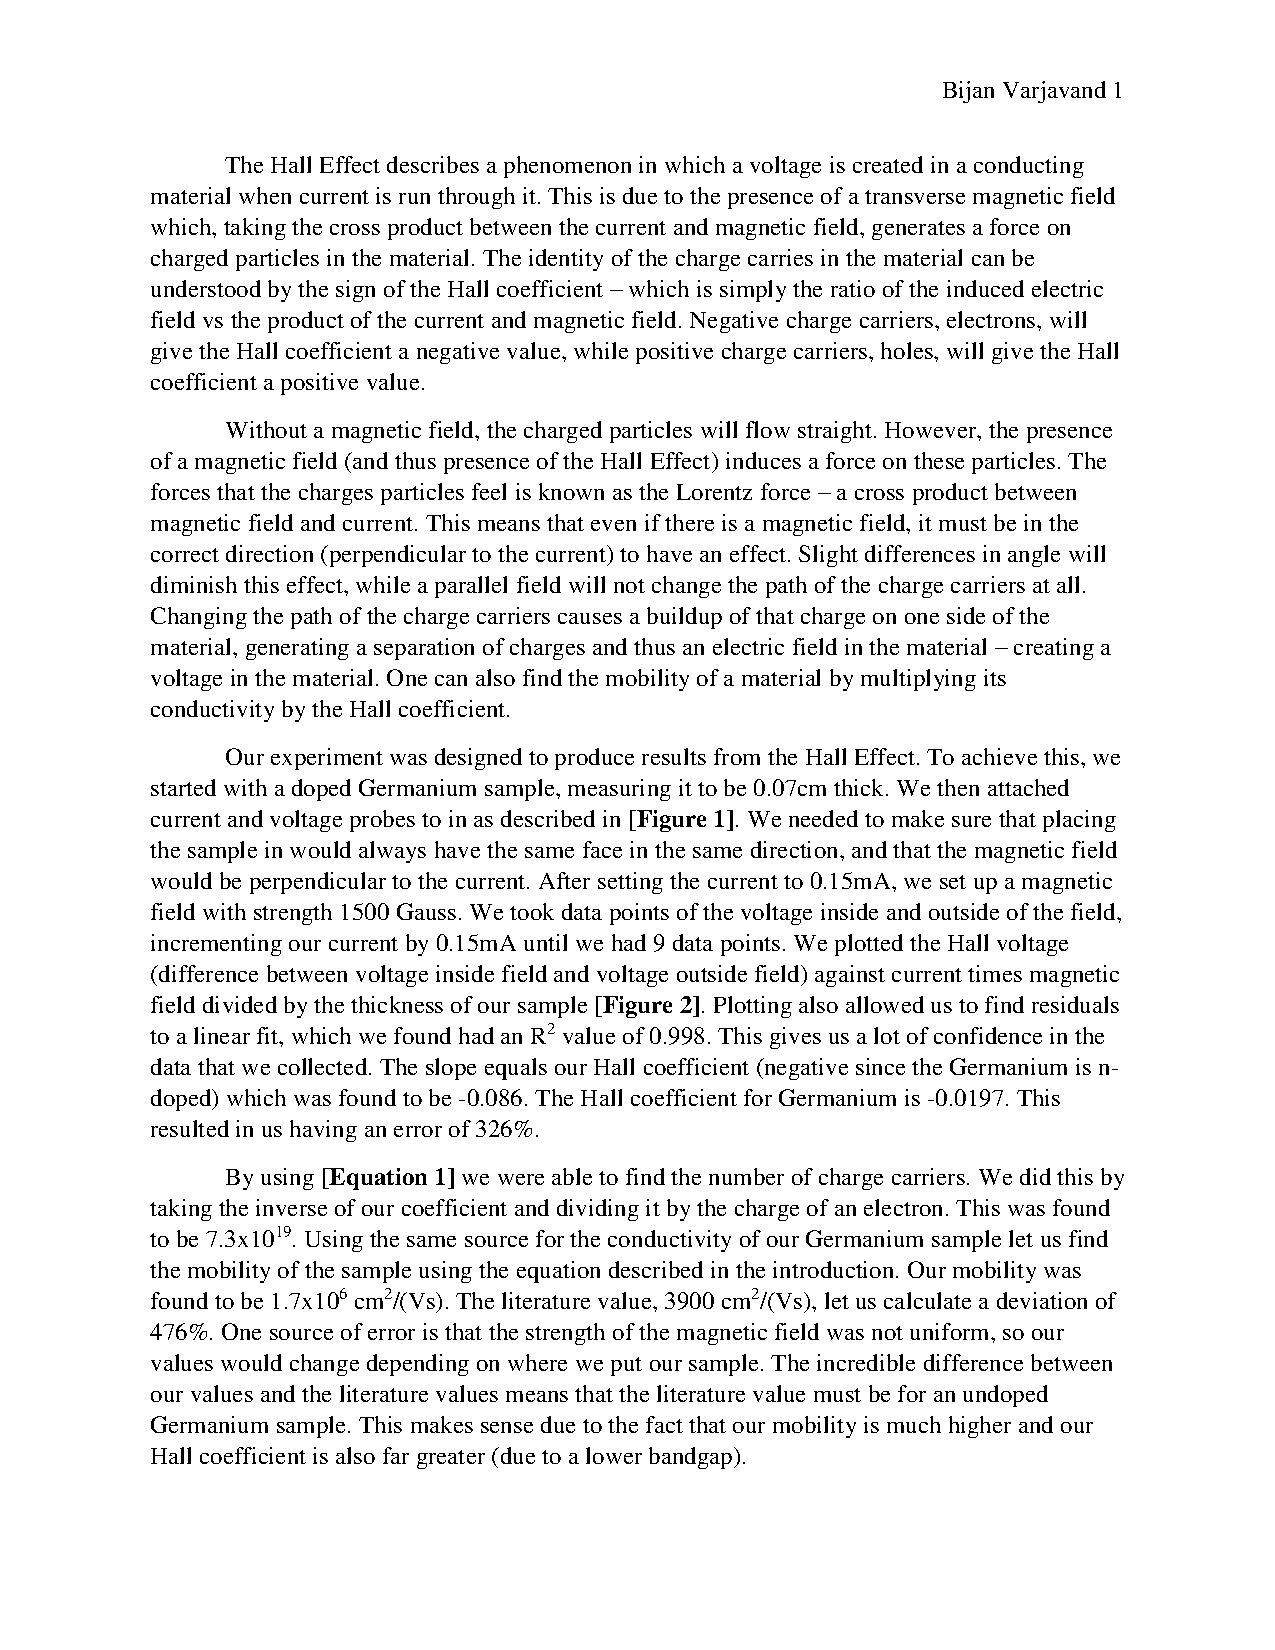
\includegraphics[scale=0.9]{hall.png}
\end{figure}

\section{Observations}

The linearization of our data is almost perfect. This verifies the equation we were given to explain the Hall effect with.

\end{document}